\section{Android app}
\label{sec:arch_app}
The app is developed to run on Android versions 4.0 or greater. As of March 2014 this makes up for 79,7\% of all Android devices in use~\cite{AndroidDeviceFragmentation}.
Support for earlier versions would require extra work, and because the app is a proof-of-concept this was not considered a problem.

The best practice guidelines for Android~\cite{androidPracticePerformance} state that one should avoid using a complex architecture. A complex architecture will increase the code base and is unnecessary in most situations. A structured pattern with concise code guidelines is needed to keep the development process as simple, effective, and bug free as possible. This section will give a detailed description of the Android app architecture. 

\subsection{Overall structure}
The Activity is the starting point of the app. It is a self contained process with the possibility to display a user interface to the user. To access the different parts of the app it was decided to use a ~\gls{navigation drawer}. The sections accessed through the navigation drawer is called a tab. The navigation drawer and all of the tabs are implemented as Fragments. A Fragment is a representation of some behavior or an interface. It is embedded inside an Activity and can be swapped in and out of the Activity. Multiple Fragments can live in the same view. A subset of the Activity life-cycle is implemented in Fragments so it can work as a self-contained module. To read more about the Android life-cycle, see the official Android documentation.~\cite{androiddoc}

\subsection{Performance}
One of the key issues in mobile app development is keeping the user interface responsive. Android renders the user interface on the main thread. Running long operations on this thread will make the interface unresponsive. Requesting data from external sources, like the server, or Facebook, is time consuming and should not run on the main thread. Handling threading correctly is critical for the overall performance of the app.

\subsection{Data access}
Data access to the underlying database is done using ContentProviders~\cite{contentproviders}. Data is accessed with \gls{URI}'s that are uniquely defined. An overview of the data layer implementation is shown in figure~\ref{fig:archAppOverview}. The view box in the figure represent the different Fragments that use data in the app. Fetching data to the view is done through the LoaderManager~\cite{loadermanager} interface. The LoaderManager loads data from the ContentProvider, and return the result asynchronously on a callback. ContentProviders used with a LoaderManager results in a view that is automatically updated when data changes, without bothering the user interface thread.

\begin{figure}[H]
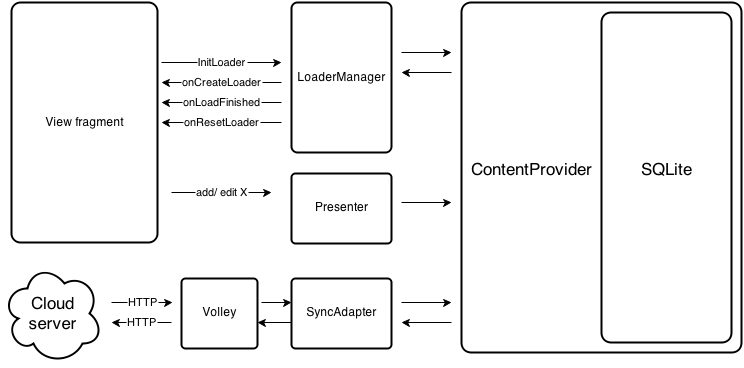
\includegraphics[width=\textwidth]{ch/architecture/fig/arch_app_overview.png}
\caption{Overview of how data is accessed}
\label{fig:archAppOverview}
\end{figure}

\newpage
\subsection{Data manipulation}
Keeping the business logic in one place makes maintaining and updating the code easier. The team decided to use the pattern Model-View-Presenter (MVP). MVP is a Model-View-Controller (MVC) derivative~\cite{mvc}. The MVP pattern separates the models, containing the data, from the presenter, handling the data, and the view, displaying the data. This is illustrated in figure~\ref{fig:mvp}. 

\begin{figure}[H]
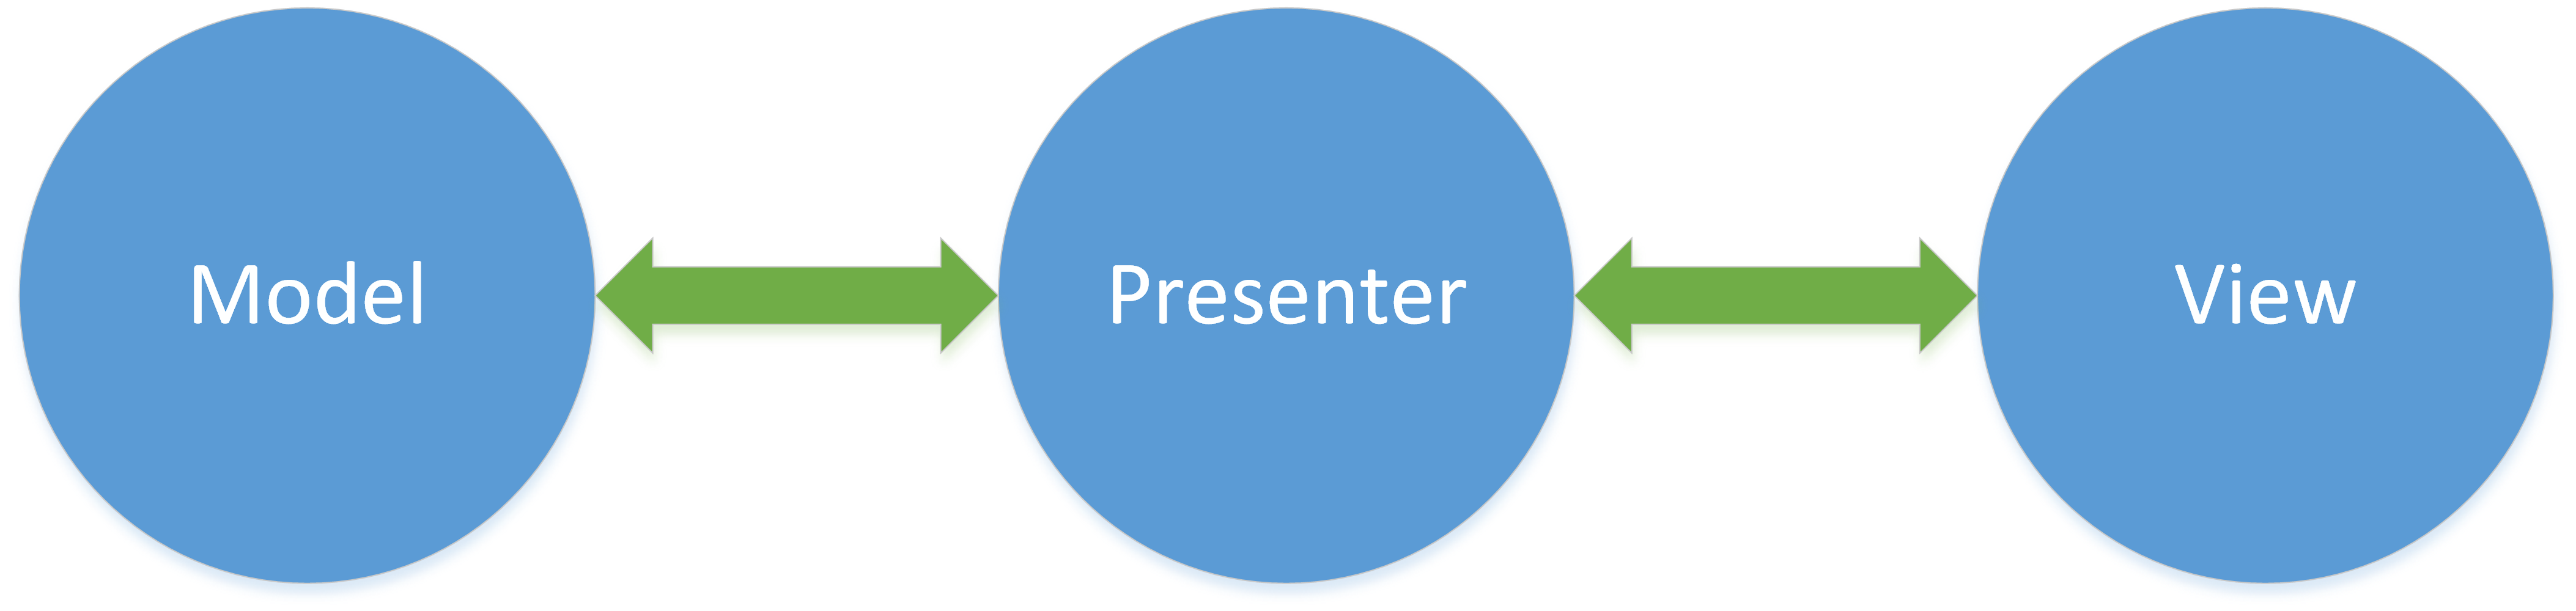
\includegraphics[width=\textwidth]{ch/architecture/fig/mvp.png}
\caption{An illustration of the Model-View-Presenter pattern}
\label{fig:mvp}
\end{figure}

\subsection{User authentication}

The system requires the user to be identified as a unique and authorized user. This authentication is done using the OAuthV2.0 protocol~\cite{oauthv2.0}. This needs a third party authenticator, in our case Facebook is used. Other OAuthV2.0 authentication providers can also be used, for instance Twitter or Google.
The Android system has its own account architecture. Working with this architecture requires the app to register an AbstractAccountAuthenticator~\cite{androidAccount} class in the AndroidManifest~\cite{androidmanifest}. When the user logs in, Facebook returns a token, stored in the AbstractAccountAuthenticator object. The token and other related user data (Facebook id) can be accessed, by the application when necessary.

\subsection{Server communication}
The app is designed with the ability to synchronize data to the server. The server, as explained in section~\ref{sec:arch_server}, exposes a restful \gls{API} were the app can retrieve and store data. Data synchronization is done by using Androids built in SyncAdapter. The SyncAdapter is an external, self-contained process that keeps the data updated. The SyncAdapter is registered to a specific account on the Android system and utilizes the ContentProvider to manipulate data. SyncAdapters can be configured to run when the system has available resources. It can also be forced to run on regular intervals.
